\section{Log GLSM (Qile Chen)}%
\label{sec:Log GLSM (Qile Chen)}

Let \(X\) be a smooth projective variety (or even a DM stack). Let \(E\) be a vector bundle on \(X\) with a section \(s \in H^0(E)\) which defines a smooth zero section \(Z\) of the expected codimension. We will refer to \(X\) and \(E\) as ambient and \(s\) and \(Z\) as the complete intersection.

\begin{quest}
    What is the relationship between the GW theory of \(Z\) and the GW theory of \((X, E)\)?
\end{quest}

When \(g = 0\), Givental and Lian-Liu-Yau used this relationship to compute the GW invariants of complete intersections, and when \(g = 1\), this was done by Zinger. In general, there are two approaches: (N)MSP and log GLSM. In this series of lectures, we will discuss log GLSM.\footnote{Qile referred the audience to the author of these notes and Yang Zhou if they have questions about MSP.}

\subsection{R-maps}%
\label{sub:R-maps}

We will consider the \textit{R-torus} \(\C^{\times}_{\omega} \coloneqq \C^{\times}\). This has a weight \(1\) representation, which we will call \(\C_{\omega}\). It descends to a line bundle \(\mc{L}_{\omega} \coloneqq [\C_{\omega} / \C^{\times}_{\omega}]\) on \(B \C_{\omega}^{\times}\). The targets of R-maps will be stacks
\[ \P \to B \C^{\times}_{\omega} \]
which are DM-type, separated, and (log) smooth. Now, an R-map consists of a (2-)commutative diagram
\begin{equation*}
\begin{tikzcd}
    & \mf{P} \ar{d} \\
    C \ar{ur}{f} \ar{r}[swap]{\omega^{\log}} \ar{d} & B \C_{\omega}^{\times} \\
    S.
\end{tikzcd}
\end{equation*}
Here, the curve could be prestable, twisted, log, or even punctured.

\begin{exm}
    Our first example is that of stable maps. Let \(\mf{P} = B\C_{\omega}^{\times}\). Because in the diagram
    \begin{equation*}
    \begin{tikzcd}
        & X \times B\C_{\omega}^{\times} \ar{d} \\
        C \ar{ur} \ar{r} & B \C_{\omega}^{\times}
    \end{tikzcd}
    \end{equation*}
    the vertical arrow is the second projection, we see that this reduces to a map to \(X\).
\end{exm}

\begin{exm}
    Consider maps
    \begin{equation*}
    \begin{tikzcd}
        & \mc{L}_{\omega} \ar{d} \\
        C \ar{ur}{f} \ar{r} & B \C_{\omega}^{\times}.
    \end{tikzcd}
    \end{equation*}
    If we assume that \(C\) is unmarked, we see that the data of this map is simply a section of \(\omega_C\), and therefore we recover holomorphic differentials.
\end{exm}

\begin{exm}
    Consider a morphism \(\C^{\times}_R \to \C^{\times}_{\omega}\) given by \(z \mapsto z^{r_{\mr{in}}}\). Then we see that
    \[ \mc{L}_R^{\otimes r_{\mr{in}}} \simeq \mc{L}_{\omega} |_{B \C_R^{\times}}. \]
    Now a diagram
    \begin{equation*}
    \begin{tikzcd}
        & B \C_R^{\times} \ar{d} \\
        C \ar{ur}{f} \ar{r} & B \C_{\omega}^{\times}
    \end{tikzcd}
    \end{equation*}
    with \(C\) unmarked is equivalent to the data of a line bundle \(\mc{L}_R|_C\) and an isomorphism \(\mc{L}_R^{\otimes r_{\mr{in}}} \simeq \omega_C\). Alternatively, we can consider R-maps of the form
    \begin{equation*}
    \begin{tikzcd}
        & \mc{L}_R \ar{d} \\
        & B \C_R^{\times} \ar{d} \\
        C \ar{uur}{f} \ar{r} & B \C_{\omega}^{\times},
    \end{tikzcd}
    \end{equation*}
    which parameterize curves with an R-spin line bundle together with a section.
\end{exm}

\begin{exm}
    Let \(X\) be a smooth projective variety. Then consider R-maps of the form
    \begin{equation*}
    \begin{tikzcd}
        & E^{\vee} \boxtimes \mc{L}_{\omega} \ar{d} \\
        & X \times B \C_{\omega}^{\times} \ar{d} \\
        C \ar{uur}{f} \ar{r} & B \C_{\omega}^{\times}.
    \end{tikzcd}
    \end{equation*}
    This is equivalent to a map \(C \to X\) together with a section \(\rho \in H^0(E^{\vee}|_C \otimes \omega_C)\).
\end{exm}

We will consider targets in the GW case.
Consider the data of an ambient \((X, E)\). Then we will set \(\mf{P}^{\circ} \coloneqq E^{\vee} \boxtimes \mc{L}_{\omega}\). The morphism \(\mf{P}^{\circ} \to B \C_{\omega}^{\times}\) is very nice, but it is not proper. To fix this, we will consider the log stack
\[ \mf{P} = ( \P(E^{\vee} \boxtimes \mc{L}_{\omega} \oplus \mc{O}) , \infty). \]
Because we have a smooth divisor in a smooth stack, the map \(\mf{P} \to B \C_{\omega}^{\times}\) is proper and log smooth. Note that we have the zero section
\[ 0_{\mf{P}} \subset \mf{P}^{\circ} \subset \mf{P} \supset \infty. \]

We will now consider targets in the r-spin case. Consider the log stack
\[ (\P(\mc{L}_R^{\oplus n} \oplus \mc{O}), \infty) = \mf{P} \to B \C_R^{\times} \to B \C_{\omega}^{\times}. \]
This morphism is proper and log smooth.

\subsection{Log and punctured R-maps}%
\label{sub:Log and punctured R-maps}

We will consider diagrams
\begin{equation*}
\begin{tikzcd}
    & \mf{P} \ar{d} \\
    C \ar{ur}{f} \ar{r}[swap]{\omega^{\log}} \ar{d} & B \C_{\omega}^{\times} \\
    S
\end{tikzcd}
\end{equation*}
where \(C \to S\) is a log or a punctured (possibly twisted) curve and \(S\) is an fs log scheme. The stability condition in the GW case is that \(f\) is representable and 
\[ (\omega_{\log})^{1+\delta} + H^{\otimes k} \otimes f^* \mc{O}(\infty) > 0 \]
for all \(0 < \delta \ll 1\) and \(k \gg 1\), where \(H\) is an ample line bundle on the coarse moduli space of \(X\). For punctured R-maps, we further require pre-stability.

\begin{exm}
    Consider the case of holomorphic differentials. Then consider \(f \in H^0(\omega_C)\) such that all zeroes are concentrated in a single Weierstrass point, where \(C\) has genus \(2\). If we consider \(\lim_{\lambda \to \infty} \lambda \cdot f\), then the limit consists of a genus \(2\) component mapping entirely to \(\infty\) and a rational component which remembers the zero.
\end{exm}

We will now discuss the tropicalization of log or punctured R-maps. Recall that a graph
\[ \ul{G} = (\V, \H, \imath \colon \H \to \H, v \colon \H \to \V) \]
consists of a set \(\V\) of vertices, a set \(\H\) of half edges, an involution \(\imath\) on the half edges, and a root map from half edges to vertices. Then we will let the set \(\L\) of legs be
\[ \L = \ab\{ h \in \H \mid \imath(h) = h\}. \]
The edges are pairs of distinct half-edges which are sent to each other by the involution:
\[ \E = \ab\{ \ab\{h, \hat{h}\} \mid \imath(h) = \hat{h} \neq h \}. \]
Now a decorated graph is a graph combined with a genus function
\[ g \colon \V \to \N, \]
an assignment
\[ r \colon \H \to \N, \]
and an ordering
\[ m \colon \L \to \ab\{0, \ldots, n\}. \]

\begin{exm}
    \leavevmode\par
    \begin{center}
    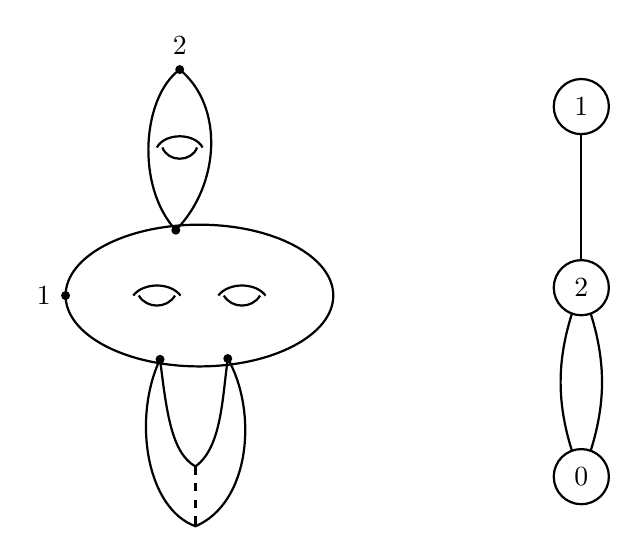
\begin{tikzpicture}[
        x=1cm,
        y=1cm,
        curve component/.style={thick},
        marked point/.style={circle,fill=black,inner sep=1.15pt},
        graph vertex/.style={
            circle,draw,thick,fill=white,minimum size=7mm,inner sep=0pt
        }
    ]
        % A three-component curve with components of genera 1, 2, and 0.
        \draw[curve component] (1.5,3.65) ellipse [x radius=1.7,y radius=0.9];

        % The two handles on the genus-two component.
        \draw[curve component]
            (0.66,3.65)
            .. controls (0.79,3.82) and (1.13,3.82) .. (1.26,3.65);
        \draw[curve component]
            (0.73,3.65)
            .. controls (0.83,3.48) and (1.09,3.48) .. (1.19,3.65);
        \draw[curve component]
            (1.74,3.65)
            .. controls (1.87,3.82) and (2.21,3.82) .. (2.34,3.65);
        \draw[curve component]
            (1.81,3.65)
            .. controls (1.91,3.48) and (2.17,3.48) .. (2.27,3.65);

        % The genus-one component attached above.
        \coordinate (uppernode) at (1.2,4.48);
        \draw[curve component]
            (uppernode)
            .. controls (0.68,5.05) and (0.78,6.18) .. (1.25,6.52)
            .. controls (1.82,6.05) and (1.76,5.05) .. cycle;
        \draw[curve component]
            (0.96,5.53)
            .. controls (1.06,5.72) and (1.44,5.72) .. (1.54,5.53);
        \draw[curve component]
            (1.03,5.53)
            .. controls (1.10,5.34) and (1.40,5.34) .. (1.47,5.53);

        % The rational component attached at two nodes below.
        \coordinate (lowerleft) at (1.00,2.84);
        \coordinate (lowerright) at (1.86,2.85);
        \draw[curve component]
            (lowerleft)
            .. controls (0.65,2.10) and (0.82,0.95) .. (1.45,0.72)
            .. controls (2.15,1.02) and (2.24,2.18) .. (lowerright);
        \draw[curve component]
            (lowerleft)
            .. controls (1.08,2.20) and (1.14,1.65) .. (1.45,1.48)
            .. controls (1.78,1.72) and (1.79,2.34) .. (lowerright);
        \draw[curve component,dashed] (1.45,1.48) -- (1.45,0.72);

        % Nodes and marked points.
        \node[marked point] at (uppernode) {};
        \node[marked point] at (lowerleft) {};
        \node[marked point] at (lowerright) {};
        \node[marked point,label=left:{$1$}] at (-0.2,3.65) {};
        \node[marked point,label=above:{$2$}] at (1.25,6.52) {};

        % The dual graph: the vertex labels record the genera.
        \coordinate (vone) at (6.35,6.05);
        \coordinate (vtwo) at (6.35,3.75);
        \coordinate (vzero) at (6.35,1.35);
        \draw[curve component] (vone) -- (vtwo);
        \draw[curve component]
            (vtwo) to[out=-112,in=112] (vzero);
        \draw[curve component]
            (vtwo) to[out=-68,in=68] (vzero);
        \node[graph vertex] at (vone) {$1$};
        \node[graph vertex] at (vtwo) {$2$};
        \node[graph vertex] at (vzero) {$0$};
    \end{tikzpicture}
    \end{center}
\end{exm}

For a log or punctured R-map
\begin{equation*}
\begin{tikzcd}
    & \mf{P} \ar{d} \\
    C \ar{ur}{f} \ar{d} \ar{r} & B \C_{\omega}^{\times} \\
    S,
\end{tikzcd}
\end{equation*}
we will tropicalize it by taking the associated generalized cone complex of the entire diagram. Because \(B \C_{\omega}^{\times}\) has no log structure, what we see is
\begin{equation*}
\begin{tikzcd}
    \Sigma(C) \ar{d} \ar{r}{\Sigma(f)} & \Sigma(\mf{P}) = \R_{\geq 0} \\
    \Sigma(S).
\end{tikzcd}
\end{equation*}
Now suppose that \(S = \Spec (Q \to \C)\) is a log point with \(Q\) an fs sharp monoid. In particular, this means that \(\Sigma(S) = Q_{\R}^{\vee}\). Because everything is (piecewise) linear, it suffices to consider an interior point \(t \in \Sigma(S)\) and consider \(\Sigma(C)_t\).

From each half edge, we treat it as pointing outward from the attached vertex, and in particular, this means that a linear map to \(\R_{\geq 0}\) corresponds to a slope. We will call these \textit{contact orders}. In particular, we have \(c(h) = - c(\hat{h})\) if \(h \neq \hat{h}\) are related by \(\imath\). For all \(v \in \V\), we also define the \textit{degeneracy}
\[ e_v \colon Q_{\R}^{\vee} \to \R_{\geq 0} \qquad t \mapsto \Sigma(f)_t (v). \]
In particular, \(e_v \in Q\) is an integral point.

The next thing we need to introduce are punctured legs. They will be denoted by
\[ \L^{\circ} = \ab\{ h \in \H \mid \Sigma(f)_t(h) \text{ is bounded and nontrivial for all } t \in Q_{\R}^{\vee}\}. \] 
We will define prestability at \(h \in \L^{\circ}\) such that \(0 \in \ol{\Sigma(f)_t(h)}\), which is a technically necessary assumption. Under the assumption that all punctured legs are prestable, we can define the \textit{edge length} function
\[ \ell \colon \E \cup \L^{\circ} \to \ms{Map}(Q_{\R}^{\vee}, \R_{\geq 0}) \qquad x \mapsto \ell(x) \colon t \mapsto \ell(x)(t). \]
Note that \(\ell(E) \in Q\) is also an integral point for edges \(E\). For punctured legs, this is true up to subdivision.

